\documentclass[compress]{beamer}

\usepackage[nofonts]{ctex}
\setCJKmainfont[ItalicFont={Kaiti SC}]{Kaiti SC}%
%\setCJKmainfont[ItalicFont={AR PL KaitiM GB}]{AR PL KaitiM GB}%
%\setCJKsansfont{WenQuanYi Zen Hei}% 文泉驿的黑体

\mode<beamer>
{
     \useinnertheme{rectangles}
     %\useoutertheme{infolines}
     %\useoutertheme{split}
     \usecolortheme{rose}
     \usecolortheme{seahorse}

     \setbeamertemplate{navigation symbols}{}%remove navigation symbols

%     \expandafter\def\expandafter\insertshorttitle\expandafter{%
%     \insertshorttitle\hfill%
%     \insertframenumber\,/\,\inserttotalframenumber}
}

\defbeamertemplate*{footline}{mytheme}
{
  \leavevmode%
  \hbox{%
  \begin{beamercolorbox}[wd=\paperwidth,ht=2.25ex,dp=1ex,center]{author in head/foot}%
    \raisebox{-1ex}{
\includegraphics[width=3ex]{Overlays/logo.pdf}}%
    \hspace*{6ex}\insertframenumber{} / \inserttotalframenumber\hspace*{2ex} 
  \end{beamercolorbox}}%
  \vskip0pt%
}
\usebeamertemplate{mytheme}

\setbeamertemplate{headline}{}

%\setbeamercovered{transparent}

\mode<handout>
{
	\usetheme{default}
	\usepackage{pgfpages}
	\pgfpagesuselayout{2 on 1}[a4paper,landscape,border shrink=5mm]
}


\usepackage{amsmath,latexsym,amssymb,amsfonts,amsbsy}
\usepackage{graphicx}
\usepackage{array}
\usepackage{hyperref}
\usepackage{textpos}
\usepackage{ulem}
\usepackage{comment}
\usepackage{fancyvrb}
\fvset{frame=single, numbers=left, fontsize=\small}
\usepackage{tikz}
\usetikzlibrary{calc,arrows.meta, graphs, trees, shapes, positioning, decorations.markings, intersections, decorations.text}
\usepackage{tikz-uml}

\newcommand{\romannumber}[1]{{\textrm{\uppercase\expandafter{\romannumeral
#1}}}}

\newcommand{\textblue}[1]{\textcolor{blue}{#1}}

\setbeamercolor{dblue}{fg=white,bg=gray!70!blue} % for beamercolorbox
 \newenvironment{pblock}{\begin{beamercolorbox}[rounded=true,
          shadow=false]{dblue}}{\end{beamercolorbox}}
 \newenvironment{bblock}{\begin{beamercolorbox}[rounded=true,
          shadow=false]{fg=black, bg=white}}{\end{beamercolorbox}}

\graphicspath{{figure/}}

%%%%%%%%%%%%%%%%%%%%%%%%%%%%%%%%%%%%%%%%%%%%%%%%%%%%%%%%%%%%%%%%%
%    body                                                       %
%%%%%%%%%%%%%%%%%%%%%%%%%%%%%%%%%%%%%%%%%%%%%%%%%%%%%%%%%%%%%%%%%


\begin{document}

%\AtBeginSubsection[]
\AtBeginSection[]
{ 
    \begin{frame}<beamer> 
		\frametitle{内容提要} 
		\tableofcontents[currentsection,currentsubsection] 
	\end{frame} 
} 

					
\title[模板方法模式]{面向对象设计模式 ~~ 模板}

\author[曹东刚]
{曹东刚\\\href{mailto:caodg@pku.edu.cn}{caodg@pku.edu.cn}}

\institute[北京大学]{北京大学信息学院研究生课程 - 面向对象的分析与设计 \\
    \href{http://sei.pku.edu.cn/~caodg/course/oo}{http://sei.pku.edu.cn/\~{}caodg/course/oo}}

\date{}

\titlegraphic{
\includegraphics[height=0.10\textwidth]{Overlays/logo.pdf}}

\begin{frame}[plain]
	\titlepage
\end{frame}

\setcounter{framenumber}{0}

%\includeonlyframes{current}

{
\defverbatim[colored]{\verbcaffee}{%
   %\renewcommand{\baselinestretch}{1.35}
\begin{Verbatim}[label=创建咖啡的代码, commandchars=\\\^\$]
public class Coffee {
  \alert^void prepareRecipe() ${ 
    boilWater();
    brewCoffeeGrinds(); 
    pourInCup(); 
    addSugarAndMilk();
  }
  public void boilWater() {}
  public void brewCoffeeGrinds() {}
  public void pourInCup() {}
  public void addSugarAndMilk() {}
}
\end{Verbatim}
}
\defverbatim[colored]{\verbtea}{%
   %\renewcommand{\baselinestretch}{1.35}
\begin{Verbatim}[label=创建茶的代码, commandchars=\\\^\$]
public class Tea {
  \alert^void prepareRecipe() ${ 
    boilWater();
    steepTeaBag(); 
    pourInCup(); 
    addLemon();
  }
  public void boilWater() {}
  public void steepTeaBag() {}
  public void addLemon() {}
  public void pourInCup() {}
}
\end{Verbatim}
}

\begin{frame}
  \frametitle{从咖啡和茶的冲泡说起}
  \only<1-2> {
  \begin{columns}
    \column{0.5\hsize}
    咖啡冲泡法:
    \begin{enumerate}
      \item 把水煮沸 
      \item 用沸水冲泡咖啡
      \item 把咖啡倒进杯子
      \item 加糖和牛奶
    \end{enumerate}
    \column{0.5\hsize}
    \pause
    茶冲泡法:
    \begin{enumerate}
      \item 把水煮沸 
      \item 用沸水浸泡茶叶
      \item 把茶倒进杯子
      \item 加柠檬
    \end{enumerate}
  \end{columns}
  }
  \only<3> {
    \verbcaffee
  }
  \only<4> {
    \verbtea
  }
\end{frame}

}

{
\defverbatim[colored]{\verbcoffee}{%
   %\renewcommand{\baselinestretch}{1.35}
\begin{minipage}[t]{0.4\hsize}
\begin{Verbatim}[label=Coffee, numbers=none, commandchars=\\\^\$]
void prepareRecipe() { 
  boilWater();
  \uline^brewCoffeeGrinds()$;
  pourInCup();
  \uline^addSugarAndMilk()$;
}
\end{Verbatim}
\end{minipage}
}

\defverbatim[colored]{\verbtea}{%
   %\renewcommand{\baselinestretch}{1.35}
\begin{minipage}[t]{0.4\hsize}
\begin{Verbatim}[label=Tea, numbers=none, commandchars=\\\^\$]
void prepareRecipe() { 
  boilWater();
  \uline^steepTeaBag()$;
  pourInCup();
  \uline^addLemon()$;
}
\end{Verbatim}
\end{minipage}
}

\defverbatim[colored]{\verbcommon}{%
   %\renewcommand{\baselinestretch}{1.35}
\begin{minipage}[t]{0.5\hsize}
\begin{Verbatim}[label=抽象后的新框架, numbers=none, commandchars=\\\^\$]
void prepareRecipe() { 
  boilWater();
  brew(); 
  pourInCup(); 
  addCondiments();
}
\end{Verbatim}
\end{minipage}
}

\defverbatim[colored]{\verbcaffeine}{%
   %\renewcommand{\baselinestretch}{1.35}
\begin{Verbatim}[label=重写CaffeineBeverage, commandchars=\\\^\$]
public abstract class CaffeineBeverage {
  \uline^final$ void prepareRecipe() {
    boilWater();
    brew();
    pourInCup();
    addCondiments();
  }
  \alert^abstract void brew()$;
  \alert^abstract void addCondiments()$;
  void boilWater() { }
  void pourInCup() { } 
}
\end{Verbatim}
}

\defverbatim[colored]{\verbnewtea}{%
   %\renewcommand{\baselinestretch}{1.35}
\begin{Verbatim}[label=重写Tea, commandchars=\\\^\$]
public class Tea extends CaffeineBeverage
{
  public void brew() { 
    System.out.println("Steeping the tea");
  }

  public void addCondiments() {
    System.out.println("Adding Lemon"); 
  }
}
\end{Verbatim}
}

\begin{frame}
\frametitle{重构,以消除重复代码}

\only<1> {
\begin{tikzpicture}
\tikzumlset{fill class=white}
\umlclass[type=abstract]{CaffeineBeverage}{}{\umlvirt{prepareRecipe()}\\ 
  boilWater() \\
  pourInCup()}
\umlclass[x=-3, y=-4]{Coffee}{}{prepareRecipe() \\
  brewCoffeeGrinds() \\
  addSugarAndMild()}
\umlclass[x=3, y=-4]{Tea}{}{prepareRecipe() \\
  steepTeaBag() \\
  addLemon()}

\umlinherit{Tea}{CaffeineBeverage}
\umlinherit{Coffee}{CaffeineBeverage}
\end{tikzpicture}
}

\only<2> {
\begin{tikzpicture}
\tikzumlset{fill class=white}
\umlclass[type=abstract]{CaffeineBeverage}{}{\umlvirt{prepareRecipe()}\\ 
  boilWater() \\
  pourInCup()}
\umlclass[x=-3, y=-4]{Coffee}{}{prepareRecipe() \\
  \alert{brewCoffeeGrinds()} \\
  \alert{addSugarAndMild()}}
\umlclass[x=3, y=-4]{Tea}{}{prepareRecipe() \\
  \alert{steepTeaBag()} \\
  \alert{addLemon()}}

\umlinherit{Tea}{CaffeineBeverage}
\umlinherit{Coffee}{CaffeineBeverage}

\umlnote[x=-3.2, width=2.5cm]{Coffee}{Coffee和Tea的特有方法算法是相同的,能否抽象?}
\end{tikzpicture}
}

\only<3> {

\noindent\begin{minipage}[t]{0.5\hsize}
\verbcoffee 
\end{minipage}%
\hspace*{-0.5\hsize}\begin{minipage}[t]{0.5\hsize}
\verbtea
\end{minipage}
}

\only<4> {
\verbcommon
}

\only<5> {
\verbcaffeine
}

\only<6> {
\verbnewtea
}
\end{frame}
}

\begin{frame}[label=current]
\frametitle{认识模板方法}
\begin{itemize}
\item CaffeineBeverage类定义并拥有算法,主导一切
\item CaffeineBeverage的模板方法提供了一个框架,允许其他子类咖啡因饮料加入
\item CaffeineBeverage专注算法本身,由子类提供完整实现
\item Coffee和Tea子类通过继承父类,复用代码
\item 算法只存在于一个地方,很容易修改
\end{itemize}
\end{frame}

{
\defverbatim[colored]{\verbabstract}{%
   %\renewcommand{\baselinestretch}{1.35}
\begin{Verbatim}[label=抽象类的设计, commandchars=\\\^\$]
abstract class AbstractClass {
  \alert^final$ void templateMethod() { 
    primitiveOperation1(); 
    primitiveOperation2(); 
    concreteOperation();
  }
  \alert^abstract$ void primitiveOperation1(); 
  \alert^abstract$ void primitiveOperation2();
  void concreteOperation() {
    // implementation here 
  }
}
\end{Verbatim}
}

\defverbatim[colored]{\verbabstracthook}{%
   \renewcommand{\baselinestretch}{1.2}
\begin{Verbatim}[label=定义了钩子的抽象类, commandchars=\\\^\$]
abstract class AbstractClass {
  \alert^final$ void templateMethod() { 
    primitiveOperation1(); 
    primitiveOperation2(); 
    concreteOperation();
    \textblue^hook()$;
  }
  \alert^abstract$ void primitiveOperation1(); 
  \alert^abstract$ void primitiveOperation2();
  void concreteOperation() {
    // implementation here 
  }
  \textblue^void hook() {}$
}
\end{Verbatim}
}

\begin{frame}
\frametitle{定义模板方法模式}

\only<1> {
\begin{block}{模板方法模式(Template Method Pattern)}
模板方法模式在一个方法中定义一个算法的骨架,而将一些步骤延迟到子类中。
模板方法使得子类可以在不改变算法结构的情况下,重新定义算法中的某些步骤
\end{block}

模板就是一个方法,该方法将算法定义成一组步骤,其中的任何步骤都可以是抽象的,
由子类负责实现
}

\only<2> {
\begin{tikzpicture}
\tikzumlset{fill class=white}

\umlclass[type=abstract]{AbstractClass}{}{templateMethod() \\
  \umlvirt{primitiveOperation1() } \\
  \umlvirt{primitiveOperation2() } 
  }

\umlclass[y=-4]{ConcreteClass}{}{
  primitiveOperation1()  \\
  primitiveOperation2()  
  }

\umlinherit{ConcreteClass}{AbstractClass}

\umlnote[x=6, width=4cm]{AbstractClass}{templateMethod $\Rightarrow$ \\
  primitiveOperation1(); \\
  primitiveOperation2();
  }

\end{tikzpicture}
}

\only<3> {
\verbabstract
}

\only<4> {
\vspace*{1ex}
\verbabstracthook
}
\end{frame}
}

{
\defverbatim[colored]{\verbcaffeinehook}{%
   \renewcommand{\baselinestretch}{1.2}
\begin{Verbatim}[label=使用钩子的CaffeineBeverage, commandchars=\\\^\$]
public abstract class CaffeineBeverageWithHook {
  final void prepareRecipe() { 
    boilWater();
    brew(); 
    pourInCup();
    \uline^if (customerWantsCondiments()) { $
      \uline^addCondiments(); $
    \uline^}$
  }
  abstract void brew(); 
  abstract void addCondiments();
\framebox^boolean customerWantsCondiments() { return true ;}$
}
\end{Verbatim}
}

\begin{frame}
  \frametitle{钩子(hook)的作用}
  \only<1> {
  \begin{itemize}
    \item 钩子是一种被声明在抽象类里的方法,但只有空的或默认的实现
    \item 钩子的存在,使得子类有能力对算法的不同点进行挂钩。要不要挂钩,
      由子类决定
    \item 如果子类必须提供算法的某个步骤,用抽象方法;如果某个步骤是可选
      的,用钩子
    \item 钩子可以让子类对模板方法中某些即将发生的步骤做出反应
  \end{itemize}
}

\only<2> {
\verbcaffeinehook
}
\end{frame}
}

\begin{frame}
\frametitle{设计原则:好莱坞原则}

\begin{block}{好莱坞原则}
别调用我们,我们会调用你
\end{block}

\begin{itemize}
\item 好莱坞原则可以防止``\uline{依赖腐败}'' --- 系统的各个构件彼此互相依赖,关系复杂,难以维护

\item 好莱坞原则使低层构件可以挂钩到系统上,但由高层构件决定何时和如何使用低层构件,即,高层构件对待低层构件是:``别调用我们,我们会调用你''
\item 模板方法模式体现了好莱坞原则
\end{itemize}
\end{frame}

{
\defverbatim[colored]{\verbarrayssort}{%
   %\renewcommand{\baselinestretch}{1.2}
\begin{Verbatim}[label=java.util.Arrays的部分排序代码, commandchars=\\\^\$]
public static void sort(Object[] a) { 
  Object aux[] = (Object[])a.clone(); 
  mergeSort(aux, a, 0, a.length, 0);
}
\end{Verbatim}
}

\defverbatim[colored]{\verbmergesort}{%
   %\renewcommand{\baselinestretch}{1.2}
\begin{Verbatim}[label=java.util.Arrays的部分排序代码, firstnumber=last, 
  commandchars=\\\^\$]
private static void mergeSort(Object src[], Object dest[], 
  int low, int high, int off)
{
  for (int i=low; i<high; i++){ 
    for (int j=i; j>low &&
      ((\alert^Comparable$)dest[j-1]).\alert^compareTo$(
        (\alert^Comparable$)dest[j])>0; j--) {
      swap(dest, j, j-1);
    }
  return; 
}
\end{Verbatim}
}

\defverbatim[colored]{\verbsortduck}{%
   %\renewcommand{\baselinestretch}{1.2}
\begin{Verbatim}[label=让鸭子支持排序, commandchars=\\\^\$]
public class Duck implements \alert^Comparable$ { 
  String name;
  int weight;
  \alert^public int compareTo(Object object)$ {
    Duck otherDuck = (Duck)object;
    if (this.weight < otherDuck.weight) { 
      return -1;
    } else if (this.weight == otherDuck.weight) { 
      return 0;
    } else 
      return 1;
  }
}
\end{Verbatim}
}

\begin{frame}
  \frametitle{Java Arrays的模板方法排序}

  \only<1> {
    \verbarrayssort
  }
  \only<2> {
    \verbmergesort
  }
  \only<3> {
    \vspace*{1ex}
    \verbsortduck
  }
\end{frame}
}

\begin{frame}
\frametitle{关于模板方法模式的小结}
\begin{itemize}
\item 模板方法定义了算法的步骤,把步骤的实现延迟到了子类
\item 模板方法模式提供了一种代码复用的重要技巧
\item 模板方法的抽象类可以定义具体方法、抽象方法和钩子
\item 抽象方法由子类实现
\item 钩子在抽象类中要么不做事,要么做缺省的事;子类可以选择是否重载他们
\item 为了防止子类改变模板方法中的算法,可以将模板方法声明为\textbf{final}
\item 好莱坞原则告诉我们,将决策权放到高层模块中,以便决定如何及何时调用低层模块
\end{itemize}
\end{frame}

\begin{frame}
\frametitle{关于设计原则的小结}
  \begin{enumerate}
    \item 封装变化
    \item 多用聚合、少用继承
    \item 针对接口编程,不针对实现编程
    \item 尽最大可能将要交互的对象设计为松耦合的
    \item 对扩展开放,对修改封闭
    \item 依赖抽象,不要依赖具体类
    \item 只和朋友交谈
    \item 别找我,我会找你
  \end{enumerate}
\end{frame}

\end{document}
